\documentclass[conference,harvard,brazil,english]{sbatex}
\usepackage[utf8]{inputenc}
\usepackage{float}
\usepackage{ae}
\usepackage{amsfonts, amssymb}
\usepackage{amsmath}
\usepackage{graphicx}
\usepackage{indentfirst}
\usepackage{ae}
\usepackage{gensymb}
\usepackage{caption} 
\usepackage{epstopdf}
\usepackage{leading}
\usepackage[shortlabels]{enumitem}
\makeatletter
\def\verbatim@font{\normalfont\ttfamily\footnotesize}
\makeatother
\usepackage{amsmath}

% --------------------------------------------------
\begin{document}
    \title{Síntese de controladores para um pêndulo invertido dinâmico}
    \author{Thalles Oliveira Campagnani}{thallescampagnani@gmail.com}
    \author{  Daniel Alves Costa}{danielac@cefetmg.br}
    \author{  Luís Felipe Silva}{luis@cefetmg.br}
    \author{  Álan Crístoffer e Sousa}{acristoffers@gmail.com}
    %--------------------------------
    \twocolumn[
        \maketitle
        \selectlanguage{brazil}
        \begin{abstract}
            O presente documento apresenta a proposta de Trabalho de Conclusão de Curso do discente de Engenharia Mecatrônica do CEFET-MG Unidade Divinópolis, Thalles Oliveira Campagnani, que é dar continuidade ao desenvolvimento ao trabalho Modelagem e Controle de Um Pêndulo Invertido Dinâmico, que vem sendo desenvolvido nas disciplinas do eixo Modelagem e Controle de Processos do curso. Para tal, é necessário realizar a modelagem/identificação do Pêndulo Invertido Dinâmico que já foi construído e utilizado no decorrer das disciplinas, realizar a síntese de controladores utilizando técnicas de controle aprendidas no decorrer do curso, realizar a simulação do sistema, e no caso dos resultados da simulação se demonstrarem promissores, aplicar no sistema real para que sejam coletados e analisados os resultados.
        \end{abstract}
        \keywords{Pêndulo invertido, síntese de controladores, modelagem de sistemas}
    ]
    \selectlanguage{brazil}
    %--------------------------------
    \section{Introdução e Contextualização}
        
        Os sistemas de controle que operam em malha aberta podem apresentar diversos problemas. Entre eles é possível destacar a falta de precisão, dinâmica lenta, instabilidade, sucessibilidade a variação de parâmetros. Com o desenvolvimento tecnológico a sociedade humana desenvolveu técnicas para realimentar os sistemas, o que permitiu que se melhorasse a resposta dinâmica, a resposta estacionaria ou tornar o sistema estável, entre outros objetivos possíveis de se atingir. Para tal, são desenvolvidos controladores, usando geralmente a diferença entre a saída desejada e a saída real do sistema para calcular a entrada, com o objetivo de tornar essa diferença nula, ou seja, que a saída real se torne a saída desejada (DORF, 2018).
        
        Um pêndulo invertido é um pêndulo que tem seu centro de massa acima de seu ponto pivô. Devido a ação da gravidade ele se torna um sistema instável, ou seja, no seu ponto de equilíbrio qualquer pertubação produzirá uma resposta divergente, derrubando o pêndulo. Sendo implementado em vários equipamentos de controle, tal experimento é útil no estudo das técnicas de estabilização e modelagem de sistema dinâmicos (Ogata, 2010). 
        
        Vários equipamentos utilizados pela sociedade no seu dia a dia podem ser modelados como pêndulos invertidos, desde brinquedos, como por exemplo um \textit{Hoverboard} a veículos automotores, como, por exemplo, uma motocicleta. % Neste ultimo caso, o da motocicleta, será chamado neste trabalho de pêndulo invertido dinâmico, pois as entrada e saída do sistema estão relacionadas a dinâmica veicular do mesmo.  
        
        A proposta para este trabalho de conclusão de curso é dar continuidade ao desenvolvimento da planta de controle Pêndulo Invertido Dinâmico, desenvolvida durante as disciplinas do eixo Controle e Modelagem de Processos do curso de Engenharia Mecatrônica do CEFET-MG unidade Divinópolis. A planta tem o formato de uma motocicleta em miniatura, possuindo duas rodas, sendo uma motora (a roda traseira), e outra para alterar a direção do veículo (a roda dianteira). Além disso, a inclinação do corpo do veículo em relação ao solo é variável, e depende indiretamente da velocidade tangencial e do angulo do eixo de direção da roda dianteira. As Figuras~\ref{motinha1} e~\ref{motinha2} permitem a visualização da planta para melhor entendimento.
        
        \begin{figure}[!ht] 
            \centering
            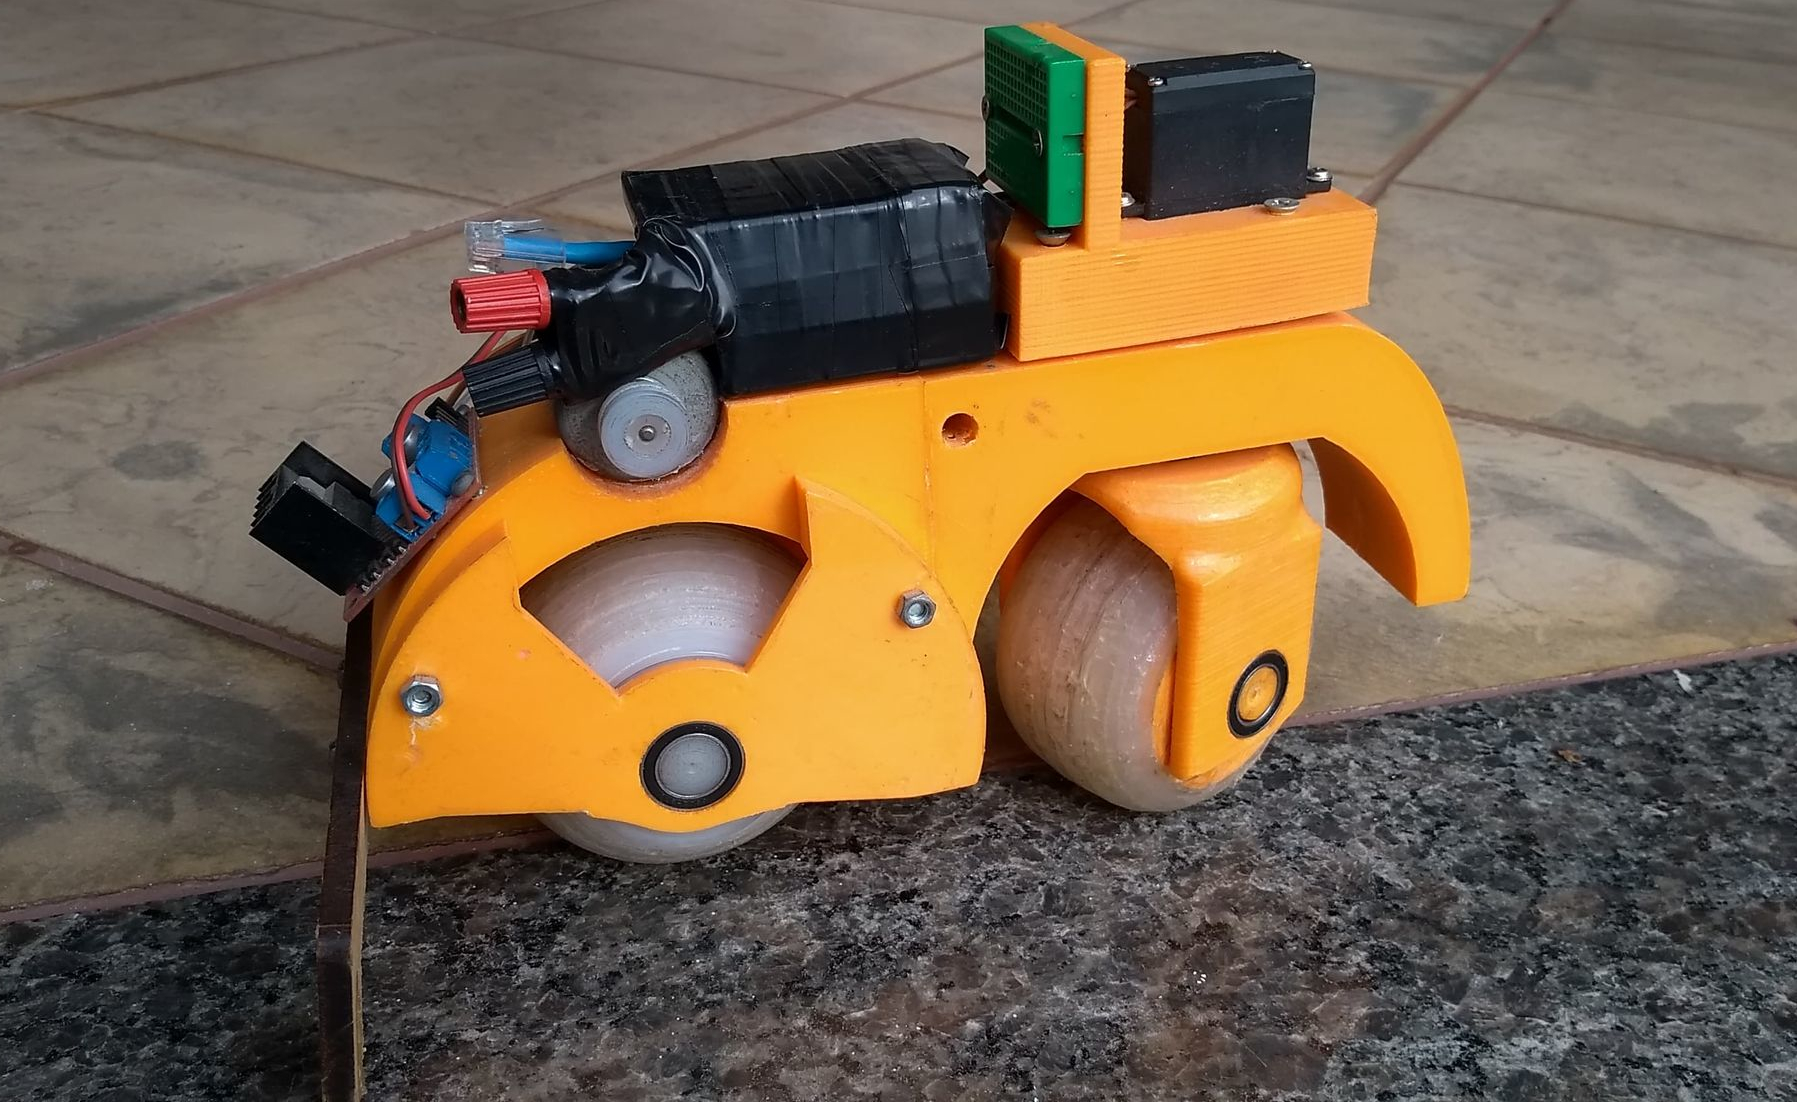
\includegraphics[width=\columnwidth]{imagens/motinha1.jpg}{
            \small
            \centering
            \caption{Vista Lateral Direita da Planta}
            \label{motinha1}}
        \end{figure}
        
        \begin{figure}[!ht] 
        \centering 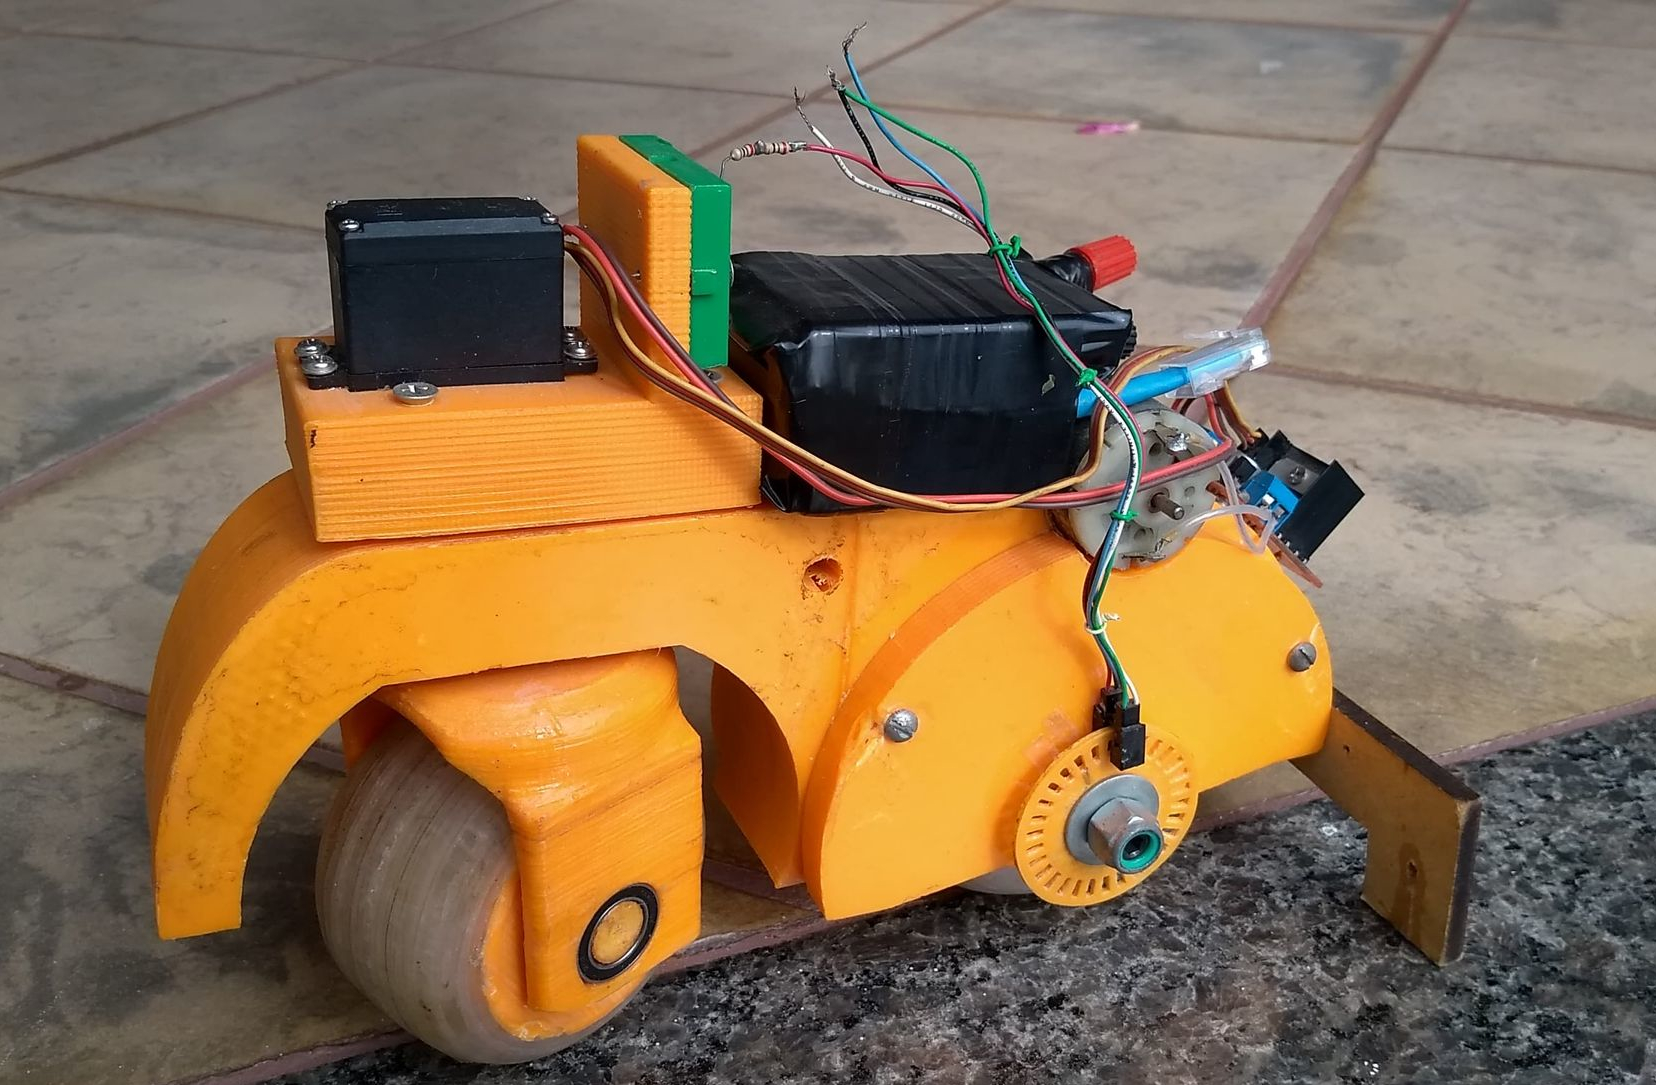
\includegraphics[width=\columnwidth]{imagens/motinha2.jpg}{
            \small
            \centering
            \caption{Vista Lateral Esquerda da Planta}
            \label{motinha2}}
        \end{figure}
        
        A planta tem como atuadores dois motores elétricos, um atuando na velocidade linear tangencial do veiculo, e outro atuando na posição do eixo de direção, logo o sistema tem duas tensões elétricas como entrada. São utilizados três sensores, um \textit{encoder} para medir a velocidade angular da roda traseira (o que é convertido em velocidade tangencial); um potenciômetro para medir a posição angular do eixo de direção; e um sensor inteligente composto de acelerômetros e giroscópios para medir a posição angular do corpo do veiculo em relação a gravidade.
        
        Como cada atuador atua em uma entrada, e cada sensor mensura uma saída, este sistema pode ser modelado como um sistema MIMO (múltiplas entradas e múltiplas saídas) sub-atuado, ou seja, a quantidade de entradas é menor que a quantidade de saídas. Além disso, é possível  dividir esse sistema em subsistemas independentes SISO (única entrada e única saída) e MISO (Múltiplas entradas e única saída) independentes, sendo esses: Sistema de velocidade tangencial; Sistema de posição angular do eixo de direção da roda; Sistema de posição angular do corpo veiculo com a gravidade. Sendo este ultimo a sistema de pêndulo invertido propriamente dito. As Figuras \ref{sistema_mimo} e \ref{sistema_sub} mostram a diferença entre as duas abordagens:
        
        \begin{figure}[!htb] 
            \centering
            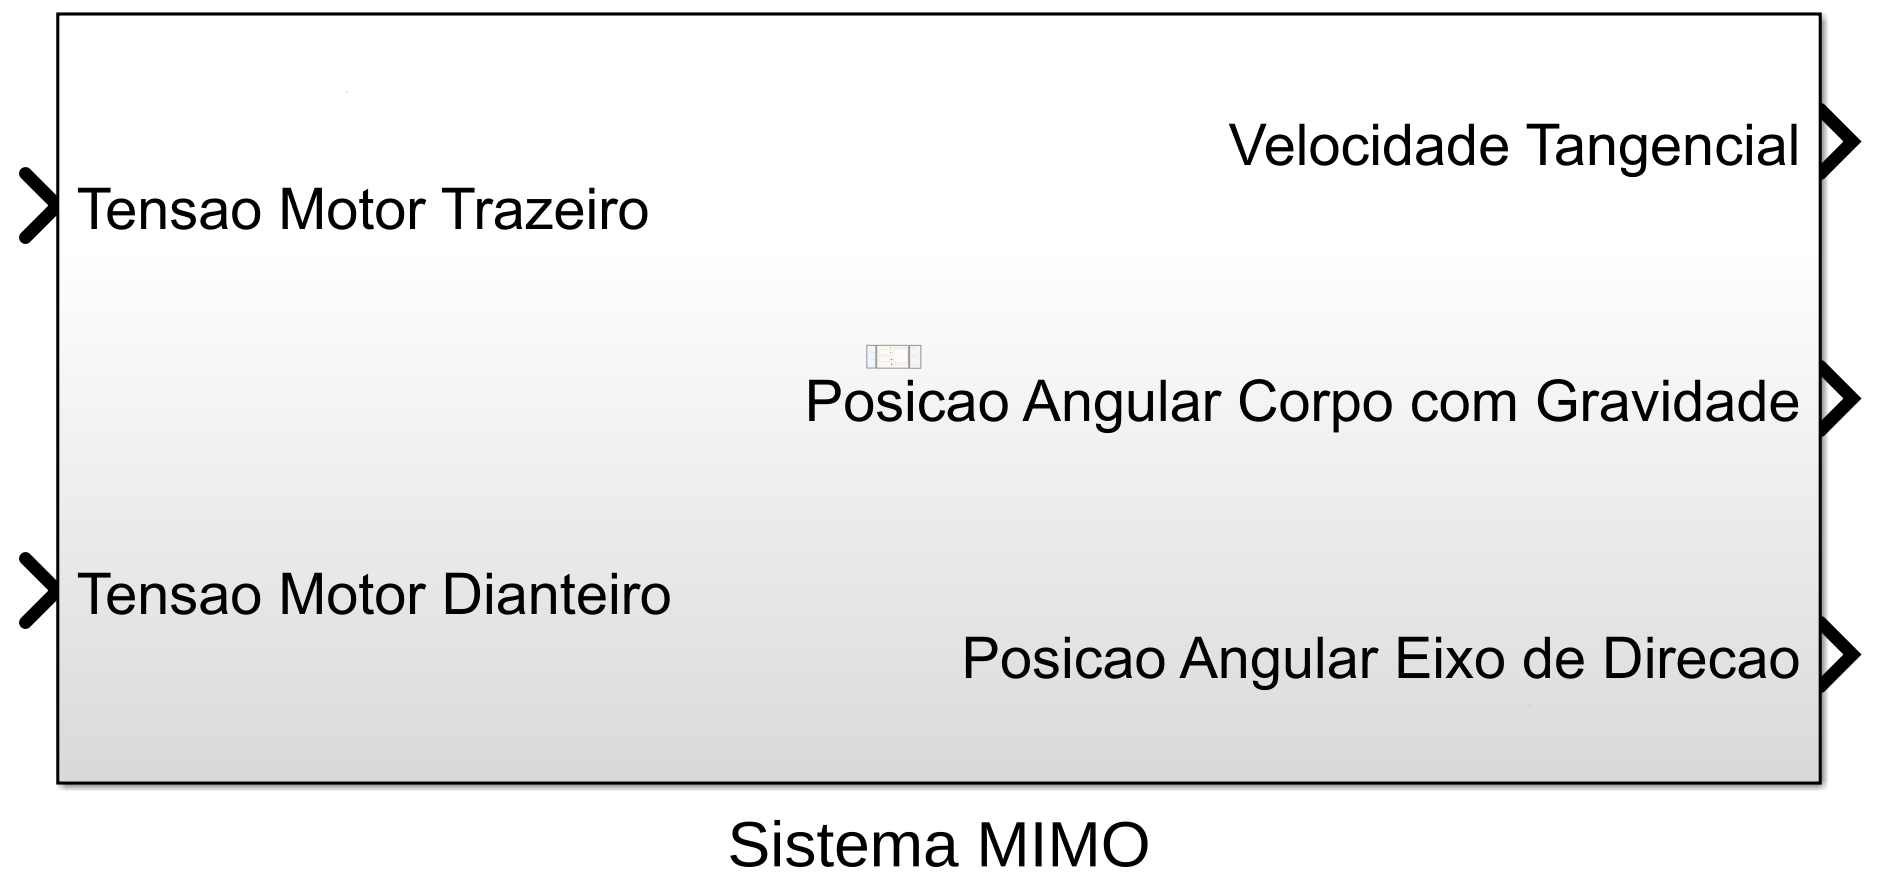
\includegraphics[width=0.7\columnwidth]{imagens/sistema_mimo.png}{
            \small
            \centering
            \caption{Modelo MIMO da planta}
            \label{sistema_mimo}}
        \end{figure}
        
        \begin{figure}[!htb] 
        \centering 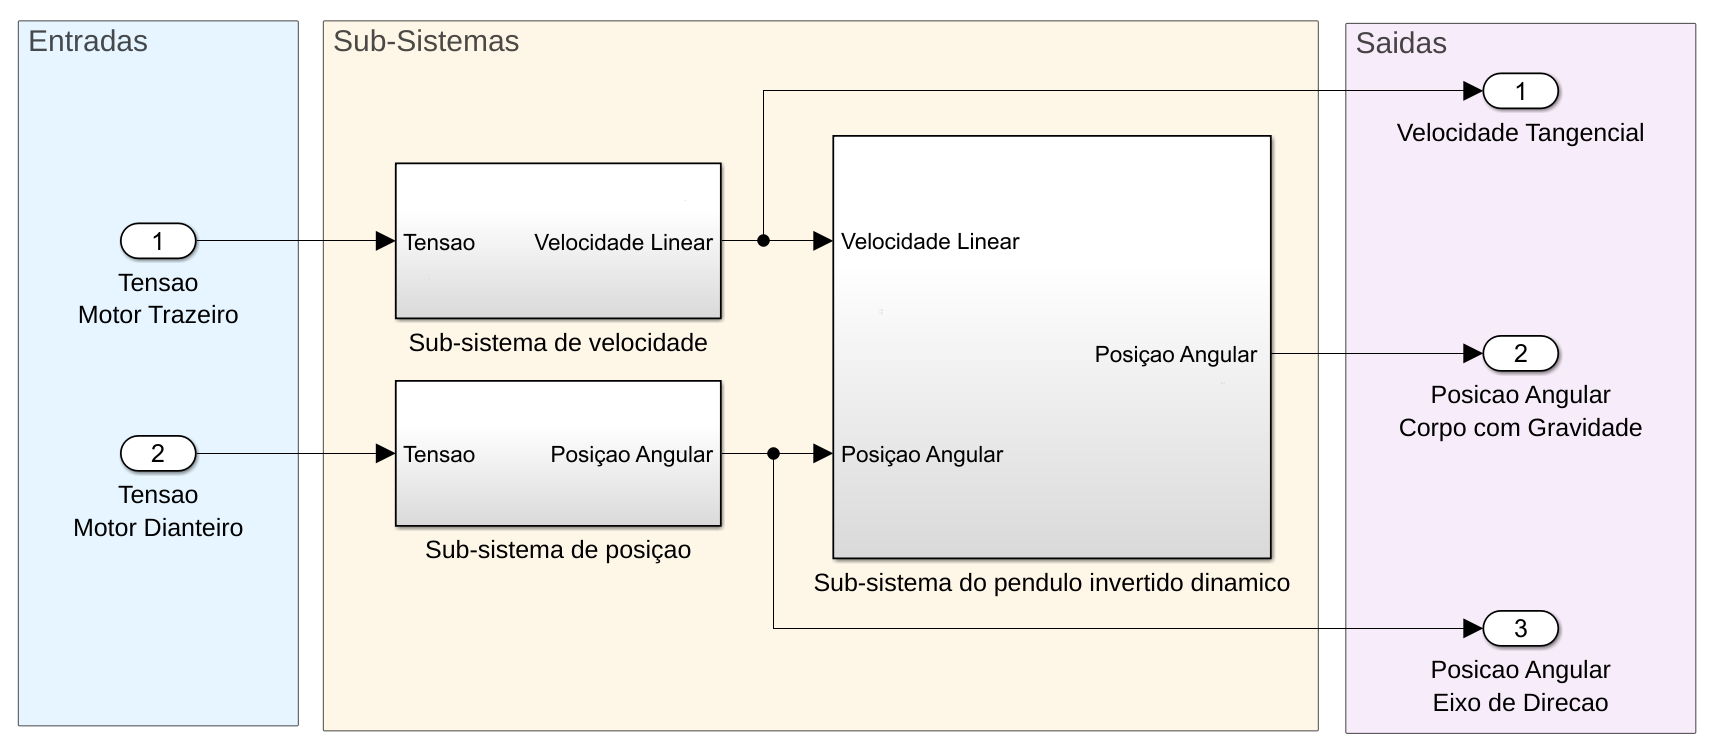
\includegraphics[width=\columnwidth]{imagens/sistema_sub.png}{
            \small
            \centering
            \caption{Planta dividida entre modelos SISO e MISO}
            \label{sistema_sub}}
        \end{figure}
        
        É preciso realizar a modelagem e/ou identificação dos subsistemas da planta, para então sintetizar controladores tendo em vista as limitações do sistema e a dinâmica desejada. Posteriormente serão realizadas simulações para comprovar se a resposta do sistema está aceitável em relação a desejada.
        
       Também será necessário desenvolver um software em que interpretará os dados dos sensores e fará o calculo do sinal de controle para os atuadores. Os dados serão coletados com o sistema real, para comprovar se a resposta está aceitável em relação a resposta desejada.
       
       Além disso, esse software deverá realizar a comunicação com um GamePad através de conexão Bluetooth, para o envio de referências para os controladores. Dessa forma, será possível controlar a velocidade e inclinação direção do veículo, e consequentemente a direção do mesmo. 
        
        \subsection{Áreas Envolvidas}
            
            A principal área deste trabalho é controle, por ter o maior peso teórico e de desenvolvimento. No entanto o trabalho também contempla a área de computação, devido a necessidade de desenvolver o software que irá executar os controladores e armazenar a aquisições de dados, e o desenvolvimento das simulações necessárias.
        
    \section{Objetivos}
    
        \subsection{Objetivos Gerais}
        
            Sintetizar controladores para a planta Pêndulo Invertido Dinâmico e desenvolver um software que execute os controladores em tempo real na planta.
        
        \subsection{Objetivos Específicos}
            
            Para atingir os objetivos gerais, é necessário realizar:
            \begin{itemize}
                \item Estudos teóricos;
                \item A integração da placa de desenvolvimento com os sensores e atuadores da planta;
                \item A modelagem e identificação dos subsistemas;
                \item A sintetização de controladores do tipo PID para os modelos obtidos;
                \item A simulação dos controladores;
                \item O desenvolvimento do software para controle da planta;
                \item Os testes dos controladores na planta e a verificação do desempenho;
            \end{itemize}
            
    \section{Metodologia}
        
        A placa de desenvolvimento precisa se comunicar com os sensores e atuadores da planta, ou seja, é necessário que seja feita a conexão eletrônica entre eles. Para isso, primeiro será desenhado o diagrama elétrico dessas conexões, depois as conexões serão realizadas e por fim serão testadas fazendo uso de ferramentas da própria placa de desenvolvimento.
        
        É preciso modelar a planta para sintetizar os controladores. O processo de modelagem será dividido em duas etapas, a primeira, a ser desenvolvida no TCC1, será a da modelagem por equações diferenciais e obtenção da função de transferência, e a segunda, a ser desenvolvida no TCC2, será a de parametrização caixa cinza nos subsistemas de velocidade e de pêndulo, e identificação e parametrização caixa preta no subsistema de direção via \textit{SISOTOOL MATLAB}, devido maior dificuldade em se modelar fisicamente ou medir certos parâmetros, como momento de inercia do subsistema.
        
        Após a validação dos modelos, serão estabelecidos critérios de desempenho observando os limites dos atuadores e sintetizados controladores do tipo PID, simulados cada um dos subsistemas separadamente usando \textit{SIMULINK}. Posteriormente esses modelos e controladores serão integrados para a simulação completa.
        
        Demonstrada a estabilidade do sistema e o atendimento aos critérios de desempenho estabelecidos, será desenvolvido o software em linguagem Python, usando a IDE Visual Studio Code, para aplicar os controladores na planta, realizar a aquisição de dados e permitir o envio de referências pelo GamePad através do Bluetooth.
        
        Após realizados os testes com os controladores aplicados na planta, os resultados serão comparados com os resultados da simulação, e serão verificados se os critérios de desempenho foram atingidos.
        
    \section{Resultados Esperados}
        
        É esperado que a resposta da velocidade tangencial da planta siga referência dada pelo \textit{gamepad} com a dinâmica projeta. E que resposta da posição angular do eixo de direção siga a referência dada pelo sinal de controle do controlador de inclinação (pendulo) também com a dinâmica projetada.
        
        A respeito da resposta do pêndulo invertido dinâmico, é esperado que siga a referencia dada pelo \textit{gamepad}, porém com oscilações aleatórias devido a grande quantidade de pertubações induzidas pelas irregularidades de superfície a qual o veículo pode percorrer.
        
        A respeito do software é esperado que ele receba as referencias do \textit{gamepad}, execute os controladores e armazene os resultados, tudo isso simultaneamente e em tempo real.
        
        E por fim, e esperado que alterando as referencias do \textit{gamepad} seja possível o utilizador controlar a velocidade e direção do veículo;
        
    \section{Recursos necessários}
        
        Todos os recursos necessários para a realização do projeto são de propriedade do discente e se encontram disponíveis para o uso, conforme lista abaixo:
        \begin{itemize}
            \item Planta de Controle: Pêndulo Invertido Dinâmico;
            \item Placa de desenvolvimento: Raspberry Pi 4;
            \item GamePad Bluetooth.
        \end{itemize}
        
       A planta de controle foi apresentada nas Figuras \ref{motinha1} e \ref{motinha2}, e a placa de desenvolvimento podem ser vistas na Figura \ref{pi}.
        
        \begin{figure}[H] 
        \centering 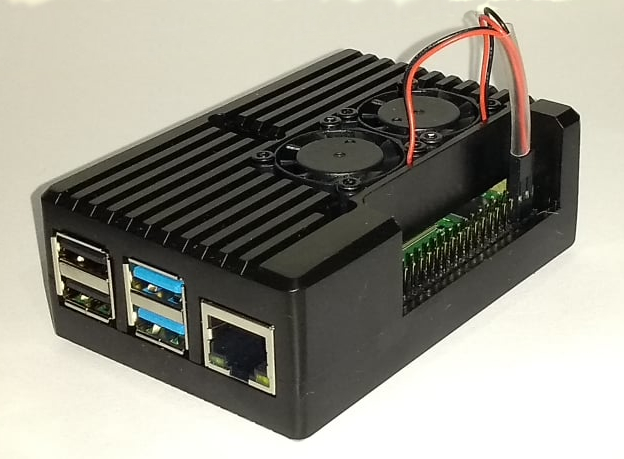
\includegraphics[width=\columnwidth]{imagens/rasp.jpg}{
            \small
            \centering
            \caption{Raspberry Pi 4 com case protetora e dissipadora de calor}
            \label{pi}}
        \end{figure}
        
    \section{Plano de trabalho}
        
        No CEFET-MG o Trabalho de Conclusão de Curso é dividido em duas etapas, o plano de trabalho será divido em entre o TCC 1 e 2. Na lista abaixo é possível ver as etapas do projeto, onde até o item 4.2) é referente ao TCC1, e até o item 10.2) é referente ao TCC2.
        
        \begin{enumerate}[1.]
            \item Estudos teóricos: 
                \begin{enumerate}[1)]
                    \item Métodos de modelagem.
                    \item Métodos de identificação.
                    \item Métodos de projeto de controladores do tipo PID.
                    \item Funcionamento do GPIO do Raspberry.
                    \item Ligação do Raspberry aos sensores e atuadores.
                    \item Programação em linguagem Python para controle.
                    \item Comunicação sem fio do Raspberry com \textit{gamepad}.
                \end{enumerate}
            \item Integração da placa de desenvolvimento com os sensores e atuadores da planta.
            \item Modelagem matemática dos subsistemas da planta e obtenção das funções de transferência.
            \item Relatório do TCC1:
                \begin{enumerate}[1)]
                    \item Escrita do relatório final de TCC1.
                    \item Defesa do TCC1.
                \end{enumerate}
            \item Parametrização dos modelos:
                \begin{enumerate}[1)]
                    \item Identificação caixa preta do subsistema de posição angular da direção da roda dianteira.
                    \item Parametrização (caixa cinza) do subsistema de velocidade da roda traseira.
                    \item Parametrização (caixa cinza) do subsistema da posição angular do corpo do veículo.
                \end{enumerate}
            \item Sintetizar controladores do tipo PID para os modelos obtidos.
            \item Simulação dos controladores:
                \begin{enumerate}[1)]
                    \item Simular separadamente os controladores aplicados nos respectivos modelos.
                    \item Simular o sistema multi variável controlado.
                \end{enumerate}
            \item Desenvolver o software para controle da planta.
            \item Testar os controladores na planta e verificar o desempenho.
            \item Relatório do TCC2:
                \begin{enumerate}[1)]
                    \item Escrita do relatório final de TCC2.
                    \item Defesa do TCC2.
                \end{enumerate}
        \end{enumerate}
        
        \subsection{Cronograma}
            
            Como não foi aprovado o calendário referente ao semestre 2021.2, foi suposto que tal semestre ocorrerá entre novembro de 2021 e fevereiro de 2022.
        
            \begin{table*}[!h]
            \caption{Cronograma de atividades}
                \begin{center}
                    \footnotesize{
                        \begin{tabular}{c|c|c|c|c|c|c|c|c}
                            \hline
                            Atividade ($\downarrow$) Mês.($\rightarrow$)    & Jun     & Jul     & Ago     & Set     & Nov     & Dez     & Jan     & Fev     \\ \hline
                            $1.1$                                           & $\surd$ &         &         &         &         &         &         &         \\ \hline
                            $1.2$                                           & $\surd$ &         &         &         &         &         &         &         \\ \hline
                            $1.3$                                           & $\surd$ &         &         &         &         &         &         &         \\ \hline
                            $1.4$                                           & $\surd$ &         &         &         &         &         &         &         \\ \hline
                            $1.5$                                           & $\surd$ &         &         &         &         &         &         &         \\ \hline
                            $1.6$                                           & $\surd$ &         &         &         &         &         &         &         \\ \hline
                            $1.7$                                           & $\surd$ &         &         &         &         &         &         &         \\ \hline
                            $2$                                             &         & $\surd$ &         &         &         &         &         &         \\ \hline
                            $3$                                             &         & $\surd$ & $\surd$ &         &         &         &         &         \\ \hline
                            $4.1$                                           &         & $\surd$ & $\surd$ &         &         &         &         &         \\ \hline
                            $4.2$                                           &         &         &         & $\surd$ &         &         &         &         \\ \hline
                            $5.1$                                           &         &         &         &         & $\surd$ &         &         &         \\ \hline
                            $5.2$                                           &         &         &         &         & $\surd$ &         &         &         \\ \hline
                            $5.3$                                           &         &         &         &         & $\surd$ &         &         &         \\ \hline
                            $6$                                             &         &         &         &         & $\surd$ &         &         &         \\ \hline
                            $7.1$                                           &         &         &         &         & $\surd$ &         &         &         \\ \hline
                            $7.2$                                           &         &         &         &         & $\surd$ &         &         &         \\ \hline
                            $8$                                             &         &         &         &         &         & $\surd$ &         &         \\ \hline
                            $9$                                             &         &         &         &         &         & $\surd$ &         &         \\ \hline
                            $10.1$                                          &         &         &         &         & $\surd$ & $\surd$ & $\surd$ &         \\ \hline
                            $10.2$                                          &         &         &         &         &         &         &         & $\surd$ \\ \hline
                        \end{tabular}
                    }
                \end{center}
            \end{table*}
            
            
    \section{Bibliografia}
        
        Åström, K. J., Murray, R. M.; Feedback Systems: An Introduction for Scientists and Engineers - 1th Edition, 2004. 
        
        Dorf, R. C; Modern Control Systems - 13th edition, 2018.
        
        OGATA, K.; Engenharia de Controle Moderno – 4ª Edição, 2010, Prentice-Hall.
        
        AGUIRRE, L. A.; Introdução a Identificação de Sistemas - 3° Edição, 2007, UFMG.
        
        "Python Software Foundation", https://www.python.org, acessado em 09/07/2021.
        
\end{document}




%%%%%%LUIS:

%Na introdução:
%As ideias dos dois primeiros parágrafos estão boas, porém precisam ser melhores escritas.
%Acredito que seja desnecessário para a proposta colocar informações muito técnicas na introdução. Melhor levá-las para a metodologia, de tal forma a mostrar ferramental necessário para tratar pontos importantes do trabalho.

%Objetivos:
%É preciso descrever de forma mais precisa os objetivos ligados a parte do desenvolvimento do software. Antes do desenvolvimento, tem a %parte de modelagem, aí precisa olhar com o Allan os termos corretos.

%Metodologia:
%Precisa apresentar 
%-as técnicas que serão utilizadas para a modelagem do sistema físico;
%-as técnicas que serão utilizadas para o projeto do controlador;
%-softwares que serão utilizados para validar;
%-as técnicas para o desenvolvimento do software;
%-as ferramentas que serão utilizadas para o desenvolvimento do software.

%Plano de trabalho:
%É preciso especificar mais. Lembre-se de associa-lo com os objetivos específicos.
%Precisa mostrar o cronograma de execução das atividades.


%%%%%%%BANCA
%O aluno não apresentou o cronograma do trabalho. 
%As bibliografias estão muito limitadas. 
%Não se tem nada sobre o desenvolvimento do software. 
%A metodologia precisa ser melhor apresentada